%%%%%%%%%%%%%%%%%%%%%%%%%%%%%%%%%%%%%%%%%%%%%%%%%%%%%%%%%%%%%%%%%%%%%%%%%%%
%%%                                                                     %%%
%%%   LaTeX template voor het verslag van P&O: Computerwetenschappen.   %%%
%%%                                                                     %%%
%%%   Opties:                                                           %%%
%%%     tt      Tussentijdsverslag                                      %%%
%%%     eind    Eindverslag                                             %%%
%%%                                                                     %%%
%%%   3 oktober 2016                                   %%%
%%%   Versie 1.4                                                        %%%
%%%                                                                     %%%
%%%%%%%%%%%%%%%%%%%%%%%%%%%%%%%%%%%%%%%%%%%%%%%%%%%%%%%%%%%%%%%%%%%%%%%%%%%

\documentclass[tt]{penoverslag}
\usepackage{url}
\usepackage{amsmath}
\usepackage{caption}
\usepackage{subcaption}
\usepackage{amsmath,bm}


%%% PACKAGES %%%



\begin{document}

% == TITELPAGINA == %
\team{Zilver}
\year{2016-2017}
\members{Bram Vandendriessche (Co\"ordinator)\\
         Arne Vlietinck (Secretaris)\\
         Matthias Van der Heyden \\
         Jef Versyck\\
         Vincent Vliegen\\
         Laura Vranken}
\maketitlepage


% == SAMENVATTING == %
\begin{abstract}
\noindent {\em Auteurs: ; redactie: Arne Vlietinck}
\\


\end{abstract}


% == INHOUDSOPGAVE == %
\tableofcontents\newpage

%Dit zal dan verwijderd worden, wanneer het verslag volledig is.
%\em Enkele algemene richtlijnen : 
\begin{itemize}
\item Maak in het hele verslag gebruik van genummerde referenties, zoals hier ge\"\i llustreerd \cite{website:wikibooks-biblio}.  
\item Geef op het niveau van secties en/of subsecties aan wie de auteurs van dat deel zijn.  Een auteur is iemand die de tekst inhoudelijk en vormelijk mee bepaald heeft.    Als de secretaris of iemand anders de tekst vormelijk gewijzigd heeft, bv. om hem meer in lijn met de rest van het verslag te brengen, maar inhoudelijk niets toegevoegd heeft, is die persoon geen auteur maar een redacteur.  Je kan na de auteursnamen eventueel ``redactie: naam'' schrijven om aan te geven dat er substanti\"ele redactie gebeurd is (meer dan pakweg een paar tikfouten verbeteren).  Wanneer alle teamleden samen verantwoordelijk zijn voor een stuk (bv. samenvatting, conclusies) kan je de namen eventueel weglaten.
\item We verwachten dat alle groepsleden een substanti\"ele bijdrage leveren aan het  verslag, en dat dit ook zichtbaar is in de tekst!
\end{itemize}


\rm 

% == INLEIDING == %
\section*{Inleiding}
\label{sec:Inleiding}
\noindent {\em Auteurs: ; redactie: Arne Vlietinck}
\\


% == Beschrijving materiaal en bouw drone == %
\section{Ontwerp}
\label{sec:Ontwerp}

\subsection{Drone Autopilot}
\label{subsec:OntwerpAutopilot}
\noindent
Ten eerste moeten de beelden die de Autopilot van de Virtual Testbed binnenkrijgt, geanalyseerd worden. Dit gebeurt door iteratief de kleurwaarden van elke pixel te vergelijken met de waarde van de opgegeven kleur. Deze methode wordt logischerwijs enkel gebruikt indien er al een doelkleur beslist is. Anders zullen de pixels gegroepeerd worden per kleur die voorkomt in een \textit{HashMap}. De gekleurde pixels worden bijgehouden door hun positie ten opzichte van het beeld, uitgedrukt in rij en kolom. De berekeningen worden gebaseerd op het midden van de bol. Dit kan benaderd worden op twee manieren: via het zwaartepunt of de kleinste-kwadratenmethode op de randpunten van de cirkel. Het zwaartepunt van een bepaalde kleur pixels is te berekenen via het gemiddelde van de opgeslagen co\"ordinaten. De kleinste-kwadratenmethode zoekt daarentegen eerst de randpunten uit van de cirkel. Deze worden vervolgens gebruikt in het zoekalgoritme (zie sectie \ref{subsec: Kleinste kwadraten circle fit}) dat de cirkel bepaalt die het beste past in de gegeven randpunten. Hieruit kan dan de positie van het centrum van de bol bepaald worden. De Autopilot zal eerst gebruik maken van de kleinste-kwadratenmethode en overschakelen op de zwaartepuntberekening wanneer er onvoldoende randpunten zijn, aangezien deze minder nauwkeurig is wanneer het middelpunt buiten beeld ligt.
\\
Indien de Autopilot geen gekleurde pixels detecteert, zal de drone systematisch de wereld scannen. Hierover meer info in sectie \ref{subsec: Scannen wereld}.
\subsection{Visuele voorstelling bij de Autopilot}
{\em Auteur: Bram Vandendriessche}\\

\noindent
Voor de grafische weergave van de gescande objecten, is een iets andere aanpak gevolgd dan bij de Polyhedra in het Testbed om een scheiding te verkrijgen tussen presentatie en representatie. \textit{TriangleAPData} bestaat louter uit de data van een Triangle, d.w.z. de co\"ordinaten van de punten en de kleuren. Een Polyhedron is opgesplitst in een data-object (\textit{PolyhedronAPData}) dat de data-driehoeken bevat, en een visueel object dat zal zorgen voor het tekenen van de driehoeken van de Polyhedron. Het visuele object bevat hiervoor een \textit{TriangleDrawer}, die d.m.v. zijn draw-methode een meegegeven \textit{TriangleAPData}-object visueel zal voorstellen.\\
~\\
\noindent
Net als het Testbed, werkt ook de Autopilot met een World, die voor de implementatie van de OpenGL-functies zorgt. De wereld werd opgesplitst in een data-object en een visueel. Dit laatste zal met de gegevens uit de data-wereld een visuele voorstelling kunnen verzorgen.\\
~\\
\noindent
Om te kunnen scannen, wat nog niet functioneel is, zullen de hoekpunten van de driehoeken omgezet worden in 3D-co\"ordinaten met behulp van de beeldherkenning. Op die manier kan een polyhedron worden samengesteld uit alle gescande driehoeken. De beeldherkenning zoekt per kleur de hoekpunten van de buitendriehoek in de linker- en rechtercamera. Om de 3D-co\"ordinaten van de hoekpunten in het wereldassenstelsel te kunnen berekenen, moeten de overeenkomstige hoekpunten uit beide beelden samengenomen worden. Het vinden van die overeenkomstige hoekpunten gebeurt door een algoritme, gelijkend op hetgeen dat controleert of een driehoek volledig is. Het zoekt eveneens naar uiterste punten en kan zo de combinaties terugvinden.  
\subsection{Ruimtelijke voorstelling d.m.v. vectoren}
\noindent {\em Auteur: Vincent Vliegen}
\\
\\
De Autopilot krijgt via de vernieuwde interface een positie en een volledige ori\"entatie mee. Deze maken het mogelijk voor de Autopilot om accuraat verplaatsingen en rotaties in de ruimte te bechrijven. De extra gegevens zorgen ervoor dat de beweging van de drone, de krachten in de ruimte en andere variabelen als vectoren kunnen beschreven worden. Ook is er voldoende informatie aanwezig om een goede benadering te maken van de effecten die de onbekende windkrachten veroorzaken.
\\
\\
De voorstelling met vectoren voorziet de mogelijkheid om het vliegtraject van de drone te bepalen en bij te sturen naar wens. De positie van de drone bepaalt enkele cruciale gegevens: de snelheid, de verplaatsingsrichting en een onbekende translatie door de wind. De ori\"entatie daarentegen is nodig om de rotaties te berekenen om de vliegrichting te corrigeren, als ook om de in- en uitwendige krachten op de drone juist te ori\"enteren en om de eventuele invloed van windrotaties in te perken. Met al deze gegevens is de Autopilot in staat om de gewenste thrust en rotatiesnelheden te bepalen, om op een zo effici\"ent mogelijke manier naar een gegeven targetpositie te vliegen.
\\
\\
Daarnaast worden objecten nu ook voorgesteld met vectoren. Aan de hand van de camerabeelden wordt de positie van het object relatief tegenover de drone bepaald. Wanneer de ori\"entatie en positie van de drone in rekening worden gebracht, is ook de positie van het object in de ruimte bekend. Deze kan dan gebruikt worden als targetpositie of voor andere doeleinden.
\subsubsection{Afremmen}
\noindent {\em Auteur: Matthias Van der Heyden}
\\
\\
De drone is zodanig ontworpen dat hij tot stilstand kan komen in de co\"ordinaten van het opgegeven target. Dit doet hij door voortdurend de targetpositie en de maximale toelaatbare acceleratie mee te geven. Deze acceleratie wordt berekend aan de hand van de drone zijn huidige snelheid en afstand tot de targetpositie.
\\
\\
Afhankelijk van zijn snelheid ten opzichte van de afstand tot het doel moet de drone afremmen (bij $\frac{snelheid}{afstand}  \geq empirische factor$) of versnellen (bij $\frac{snelheid}{afstand}  < empirische factor$). De grootte van de acceleratie of deceleratie is steeds de maximaal mogelijke waarde, rekening houdend met de huidige wind, tenzij de afstand tot het doel kleiner is dan een bepaalde afstand. In dat geval verkleint de waarde met een afstandsafhankelijke factor.
%TODO: polyhedra calculation -> @Laura
%TODO: scannen 1) tekenen; 2) idee -> @Bram & @Laura

\subsection{Virtual Testbed}
%TODO: Tekenen polyhedron -> @Bram
\subsection{Polyhedra en het bestaande ontwerp}
\noindent {\em Auteur: Bram Vandendriessche}
\\\\
Het ontwerp van de simulator zorgt ervoor dat de uitbreiding ervan met polyhedra vrij eenvoudig in te voeren is. Door het nieuwe type Polyhedron dat erft van de \textit{WorldObjects}, moesten in \textit{World} zelf slechts enkele extra methodes worden ge\"implementeerd m.b.t. het toevoegen en verwijderen van een Polyhedron aan de bestaande wereld.\\
\noindent
Het ontwerp van het Testbed heeft de grote zwakte dat het erg moeilijk is om individuele elementen en methodes te testen. Dit komt doordat de objecten vaak erg afhankelijk zijn van de wereld waarin ze bestaan. Die wereld is bovendien altijd afhankelijk van de \textit{gl}-component van OpenGL, waardoor het noodzakelijk is een volledige wereld op te zetten voor de test kan worden uitgevoerd. Een oplossing hiervoor zou zijn om de objecten en wereld zo op te splitsen dat presentatie en representatie gesplitst worden, zodat het representatie-gedeelte onafhankelijk kan gebruikt worden. Daarnaast zou dan enkel de wereld weet moeten hebben van haar objecten en niet andersom, zodat objecten onafhankelijk van de wereld kunnen worden getest.\\
\\
\noindent 
De Polyhedron zelf is zo ontworpen dat die bestaat uit verschillende Triangles. De tekenfunctie van de Polyhedron draagt elke Triangle die tot de Polyhedron behoort, op om zichzelf te tekenen. Een Triangle bestaat uit co\"ordinaten voor zijn drie hoekpunten en een kleur voor het buitenste gedeelte van de driehoek. Op basis daarvan worden de binnenste hoekpunten berekend en er wordt een kleur afgeleid uit de gegeven kleur zodat de driehoek voldoet aan de gegeven beperkingen m.b.t. de kleur, zie Tabel \ref{table: HSVwaarden}, en de oppervlakte.\\
\\
\noindent
Voor het testen van de Autopilot zijn verschillende figuren ontworpen. Zij vallen onder de \textit{PredefinedPolyhedron}, een subklasse van Polyhedron die ook een positie mee kan krijgen bij creatie. Hierdoor kan de figuur op een gewenste positie worden geplaatst. De standaard Polyhedra krijgen geen positie mee. Hun positie wordt gezet op het massapunt van de polyhedron (de gemiddelde 3D-co\"ordinaat van alle hoekpunten). Op die manier wordt gezorgd dat de positie logisch is t.o.v. de hoekpunten en het niet mogelijk is dat een figuur bijvoorbeeld rond (20,0,0) wordt gedefinieerd, maar wel een positie van (0,0,-40) krijgt toegewezen. De figuren vari\"eren van een eenvoudige met vier hoekpunten tot meer complexe zoals een kubus met een opening in, waarbij de Autopilot zal moeten weten dat het voor de drone niet mogelijk is hierdoor te vliegen, zie Figuur \ref{fig: polyhedra}.

\begin{figure}[h]
	\centering
	\begin{subfigure}{.5\textwidth}
		\centering
		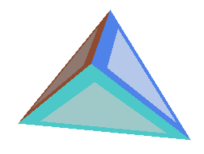
\includegraphics[width=.4\linewidth]{4point.png}
		\caption{Eenvoudige figuur}
	\end{subfigure}%
	\begin{subfigure}{.5\textwidth}
		\centering
		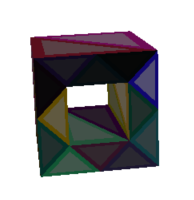
\includegraphics[width=.4\linewidth]{hollowcube.png}
		\caption{Complexere figuur}
	\end{subfigure}
	\caption{Voorgedefinieerde polyhedra.}
	\label{fig: polyhedra}
\end{figure}

%TODO: Generator/parser -> @Jef
\subsubsection{Generator en editor}
Daarnaast werd er ook dit semester gevraagd om een wereld generator zelf te implementeren. Elk bestand gegenereerd door deze generator, moest voldoen aan de opgestelde eisen. Op dit moment zijn er twee generators, één die een wereld met bollen maakt en één die een wereld met Polyhedra maakt. Deze laatste kiest uit verschillende vooraf aangemaakte vaste Polyhedra, zoals hierboven vermeld.
\\

\noindent
Verder is de editor verder uitgewerkt. Men selecteert eerst een object met behulp van de muis. Met behulp van de toetsen i en k (bewegen volgens positieve en negatieve x-as), j en l (bewegen volgens positieve en negatieve z-as), u en o (bewegen volgens positieve en negatieve y-as), kan elk object nu verplaatst worden in de wereld. Er bestaat op dit moment geen manier om polyhedra toe te voegen. Elk object kan verwijderd worden met behulp van de DELETE knop.


% == ALGORITMES == %
\section{Algoritmes}
\label{sec:Algoritmes}

\subsection{Drone Autopilot}
\label{sec:AlgoritmesAutopilot}
%RotatieMatrixen
\subsubsection{Rotatiematrix}
\noindent {\em Auteur: Laura Vranken; redactie: Arne Vlietinck}
\\\\
Na een uitgebreide wijziging van de opgave werden de rotatiematrixen opnieuw opgesteld. De conventies in de nieuwe opgave komen niet overeen met de algemene conventies in de literatuur. Hierdoor werden de rotatiematrixen met extra zorg opgesteld. Het is een cruciaal element voor de ori\"entatie en bewegingen van de drone.

\begin{figure}[h!]
	\centering
		\(
		\begin{bmatrix} 
			cos(y) & 0 & -sin(y) \\ 
			0 & 1 & 0 \\
			sin(y) & 0 & cos(y)
		\end{bmatrix}
		\begin{bmatrix} 
			1 & 0 & 0 \\ 
			0 & cos(p) & sin(p) \\
			0 & -sin(p) & cos(p)
		\end{bmatrix}
		\begin{bmatrix} 
			cos(r) & sin(r) & 0 \\ 
			-sin(r) & cos(r) & 0 \\
			0 & 0 & 1
		\end{bmatrix}
		\)
	\caption{Bovenstaande matrixen geven respectievelijk de yaw-, pitch- en rollmatrix weer.}
\end{figure}
\noindent
Bovenstaande matrixen worden vermenigvuldigd in omgekeerde volgorde dit door de conventies van de rotatiematrixen. Met deze rotatiematrix kan ook de inverse berekend worden.\label{key}
\subsubsection{Vliegstrategie}
\noindent {\em Auteur: Vincent Vliegen}
\\
\\
De autopilot maakt gebruik van vectoren om de drone en andere objecten in de ruimte te situeren. Dit maakt het mogelijk om de thrustgrootte en rotatiesnelheden te berekenen, zodat we vliegen volgens een optimaal pad.
\\
\\
De drone start met een gegeven positie en ori\"entatie. De autopilot heeft nu twee opties. Oftewel stelt deze in dat de drone naar een andere positie in de ruimte vliegt, oftewel dat de camera's anders geori\"enteerd worden.
\\
Omwille van de uitwendige krachten op de drone vliegt de drone niet in de richting van de thrustkracht. De zwaartekracht, de drag en de wind, berekend en opgeteld met de thrust, resulteren samen in de verplaatsingsrichting van de drone. Wanneer er een targetpositie is meegegeven, kan de thrustgrootte dan ook zo ingesteld worden, dat de drone zo goed mogelijk in de richting van het doel vliegt.
\\
\\
Daarna wordt een gewenste ori\"entatie berekend. Hiervoor bestaan meerdere opties. Enerzijds kunnen de camera's een gevraagde richting uit kijken met de thrust zo gericht dat de drone het beste stil hangt. Anderzijds kan de thrust zo ingesteld worden dat de drone met een gewenste versnelling naar een doel vliegt en de camera's dat ze zo goed mogelijk kijken volgens het vliegtraject.
\\
Wanneer de gewenste ori\"entatie bekend is, kunnen de nodige rotatiesnelheden berekend worden om de drone bij te sturen. Met behulp van de rotatiematrices worden de nog af te leggen rotaties bepaald. Als hierbij het benaderde rotationele effect van de wind mee in rekening word gebracht, kunnen de rotatiesnelheden voor de yaw, pitch en roll vastgelegd worden.
\subsubsection{Wind correctie}
\noindent {\em Auteur: Vincent Vliegen}
\\
\\
De wind zorgt voor een verandering op de positie en ori\"entatie van de drone. Aangezien de Autopilot wordt opgeroepen onder een constant tijdsinterval, kunnen er voorspellingen worden gemaakt over de ruimtelijke situering van de drone, wanneer er een bepaalde hoeveelheid tijd is verlopen.
\\
\\
De Autopilot stelt de thrust en de rotatiesnelheden in. Met behulp van de uitwendige krachten en rotaties kunnen de verplaatsingsrichting en verandering van ori\"entatie bepaald worden. Wanneer ook het constante tijdsinterval in rekening wordt gebracht, kan de verwachte positie benaderd worden aan de hand van de bewegingsvergelijking:
\begin{equation}
	 \frac{(\vec{T} + \vec{G} + \vec{D} + \vec{W}) }{2m} * (\Delta t)^2 + \vec{v_0} * \Delta t + \vec{x_0} = \vec{x}_{exp}
\end{equation}
De verwachtte yaw, pitch en roll, die samen de ori\"entatie bepalen, worden als volgt berekend:
\begin{equation}
	\theta_0 + (\omega + \omega_{wind})*\Delta t = \theta_{exp}
\end{equation}
\\
De Autopilot controleert in het begin van elke cyclus of de verwachte positie en de eigenlijke positie overeenkomen, respectievelijk de verwachte en eigenlijke ori\"entatie. Zo niet, is de afwijking te verklaren als een verandering van de windtranslatie en -rotatie. 
\\
Het verschil in positie is het gevolg van een onnauwkeurige benadering van de windtranslatie. Deze kan gecorrigeerd worden door de kracht te berekenen die de afwijking heeft veroorzaakt, en dan op te tellen bij de huidige windkracht.
\begin{equation}
	\frac{(\vec{W}_{corr}) }{2m} * (\Delta t)^2 = \vec{x}-\vec{x}_{exp}
\end{equation}
De afwijking in rotatie duidt een rotatieverandering van de wind aan. Ook hier kan een correctie berekend worden voor de yaw, pitch en roll, die vervolgens opgeteld wordt met de huidige windrotaties.
\begin{equation}
	\omega_{corr}*\Delta t = \theta-\theta_{exp}
\end{equation}

\subsection{Virtual Testbed}
\subsection{Collision Detection}
\noindent {\em Auteur: Jef Versyck}
\\\\
Aangezien polyhedra niet per definitie mooie cirkels zijn, moet de collision detection veranderd worden. Eerst wordt er vergeleken of de afstand tussen de twee centra van de objecten (een polyhedron en de drone) kleiner is dan beide hun radii opgeteld. De radius van een polyhedron wordt gedefiniëerd als de grootste afstand tussen het centrum van de polyhedra en zijn punten. \\
\noindent
Vervolgens wordt er getest of de loodrechte afstand op het vlak van een Triangle vanuit het middelpunt van de drone kleiner is dan de straal van de drone. Hierbij wordt het vlak waarin de Triangle zich bevindt, berekend aan de hand van het kruisproduct van twee vectoren van de Triangle en een hoekpunt ervan. Vervolgens wordt de loodrechte projectie op het vlak bepaald. Dit punt heet P. In formulevorm: 
\begin{gather*}
	a\cdot x + b\cdot y + c\cdot z = d \\ 
	t = -\frac{a \cdot x_{drone} + b \cdot y_{drone} + c \cdot z_{drone} - d}{a^2 + b^2 + c^2}  \\ P =
	\begin{Bmatrix}
	a\cdot t + x_{drone}\\ 
	b\cdot t + y_{drone}\\ 
	c\cdot t + z_{drone}
	\end{Bmatrix}
\end{gather*}

\noindent
 Dit is echter niet genoeg. De loodrechte projectie van het massacentrum  kan zich buiten de Triangle bevinden en zo een foutief resultaat geven. Om te zien of het punt zich binnen de Triangle bevindt, wordt aan de hand van barycentrische coördinaten gecontroleerd. Het principe hierachter is dat elk punt P in de driehoek geschreven kan worden als een lineaire combinatie van de hoekpunten (A, B en C) van een driehoek. De som van alle co\"effici\"enten moet gelijk zijn aan één en alle co\"effici\"enten moeten groter zijn dan nul. In formulevorm:
 
 \begin{gather*}
 	P = u\cdot A + v\cdot B + w\cdot C \\
 	0 \le u,v,w \le 1 \\
 	u + v + w = 1
 \end{gather*}

%TODO https://www.scratchapixel.com/lessons/3d-basic-rendering/ray-tracing-rendering-a-triangle/barycentric-coordinates hierbij als referentie zetten

\noindent
Dit lost echter niet alle problemen op. De drone kan de polyhedron raken, maar de loodrechte afstand kan buiten de triangle liggen. Hiervoor werd ten tijde van schrijven nog geen oplossing gevonden. Zie Figuur \ref{fig:CollisionDetectionProbleem} voor verduidelijking. Het snijpunt ligt duidelijk buiten de Triangle, maar toch snijdt de drone de Triangle.
\begin{figure}[h]
	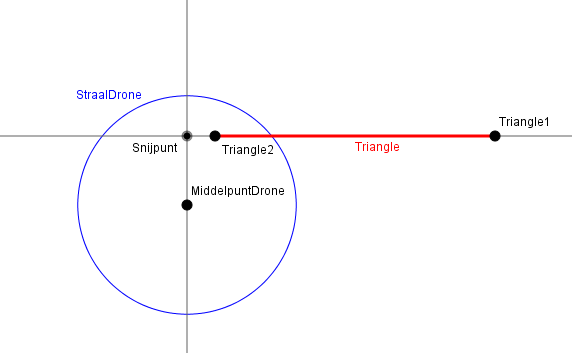
\includegraphics[width=1\textwidth]{CollisionDetectionProbleem.png}
	\caption{Een voorbeeld van het probleem met de huidige collision detection.\\ }
	\label{fig:CollisionDetectionProbleem}
\end{figure}

% == SOFTWARE == %
\section{Software}
\label{sec:Software}

\subsection{Drone Autopilot}

\subsection{Virtual Testbed}


% == Testen == %
\section{Testen}
\label{sec:Testen}
\subsection{Testen beeldverwerking}
\noindent {\em Auteur: Laura Vranken}
\\\\
Om de beeldverwerking van de polyhedra te testen, zijn verschillende afbeeldingen in het project ingeladen. Hierop zijn verschillende testen uitgevoerd. Er wordt onder andere gecontroleerd of de omzetting van integer waarden naar HSV waarden juist gebeurt. Bovendien is ook de functie getest die het zwaartepunt van elke zichtbare volledige driehoek teruggeeft. Dit bleek vrij accuraat.
\\
De laatste test controleert of het bepalen van de 3D co\"ordinaten van de hoekpunten juist gebeurt. Dit is geverifieerd met de co\"ordinaten van het Testbed.

% == BESLUIT == %
\section*{Besluit}
\label{sec:Besluit}
\noindent {\em Auteurs: ; redactie: Arne Vlietinck}
\\

% == REFERENTIES == %
\bibliographystyle{siam}
\bibliography{references.bib}


% == APPENDICES == %
%\newpage\makeappendix


%\section{MOET NOG WEG}
%De volgende informatie wordt na de finale demonstratie apart ingediend.

\section{Beschrijving van het proces}
\begin{itemize}
\item Welke moeilijkheden heb je ondervonden tijdens de uitwerking?
\item Welke lessen heb je getrokken uit de manier waarop je het project hebt aangepakt?
\item Hoe verliep het werken in team? Op welke manier werd de teamco\"ordinatie en planning aangepakt?
\end{itemize}


\section{Beschrijving van de werkverdeling}
\begin{itemize}
\item Geef voor elk van de groepsleden aan aan welke delen ze hebben meegewerkt en welke andere taken ze op zich hebben genomen.
\item Rapporteer in tabelvorm hoeveel uur elk groepslid elke week aan het project gewerkt heeft, zowel tijdens als buiten de begeleide sessies. Geef ook totalen per groepslid voor het volledige semester.
\end{itemize}


\section{Kritische analyse}
\begin{itemize}
\item Maak een analyse van de sterke en zwakke punten van het project. Welke punten zijn vatbaar voor verbetering. Wat zou je, met je huidige kennis, anders aangepakt hebben?
\end{itemize}



\end{document}
